\section{Implementation}
In this section, we describe the implementation of \system and discuss its remaining limitations.
\subsection{Plugin Architecture}
We implement \system as a backend-agnostic plugin layer rather than tightly integrating it into a specific ANNS backend. Each backend is connected through a lightweight adapter that exposes a unified interface for index setup, insertion, deletion, and query execution. \system does not modify the backend's index construction, update policy, or original search procedure; all seed management logic is implemented outside the backend core. To ensure fair and reproducible evaluation, the same benchmark pipeline is used for both the original backend and its \system-enabled variant under identical workloads and system settings. Deployment parameters, such as the high-utility capacity, the number of semantic-shared buckets, and the per-bucket seed capacity, are externalized in configuration files and logged together with dataset, batch, and backend settings at startup.
\begin{figure*}[t]
\centering
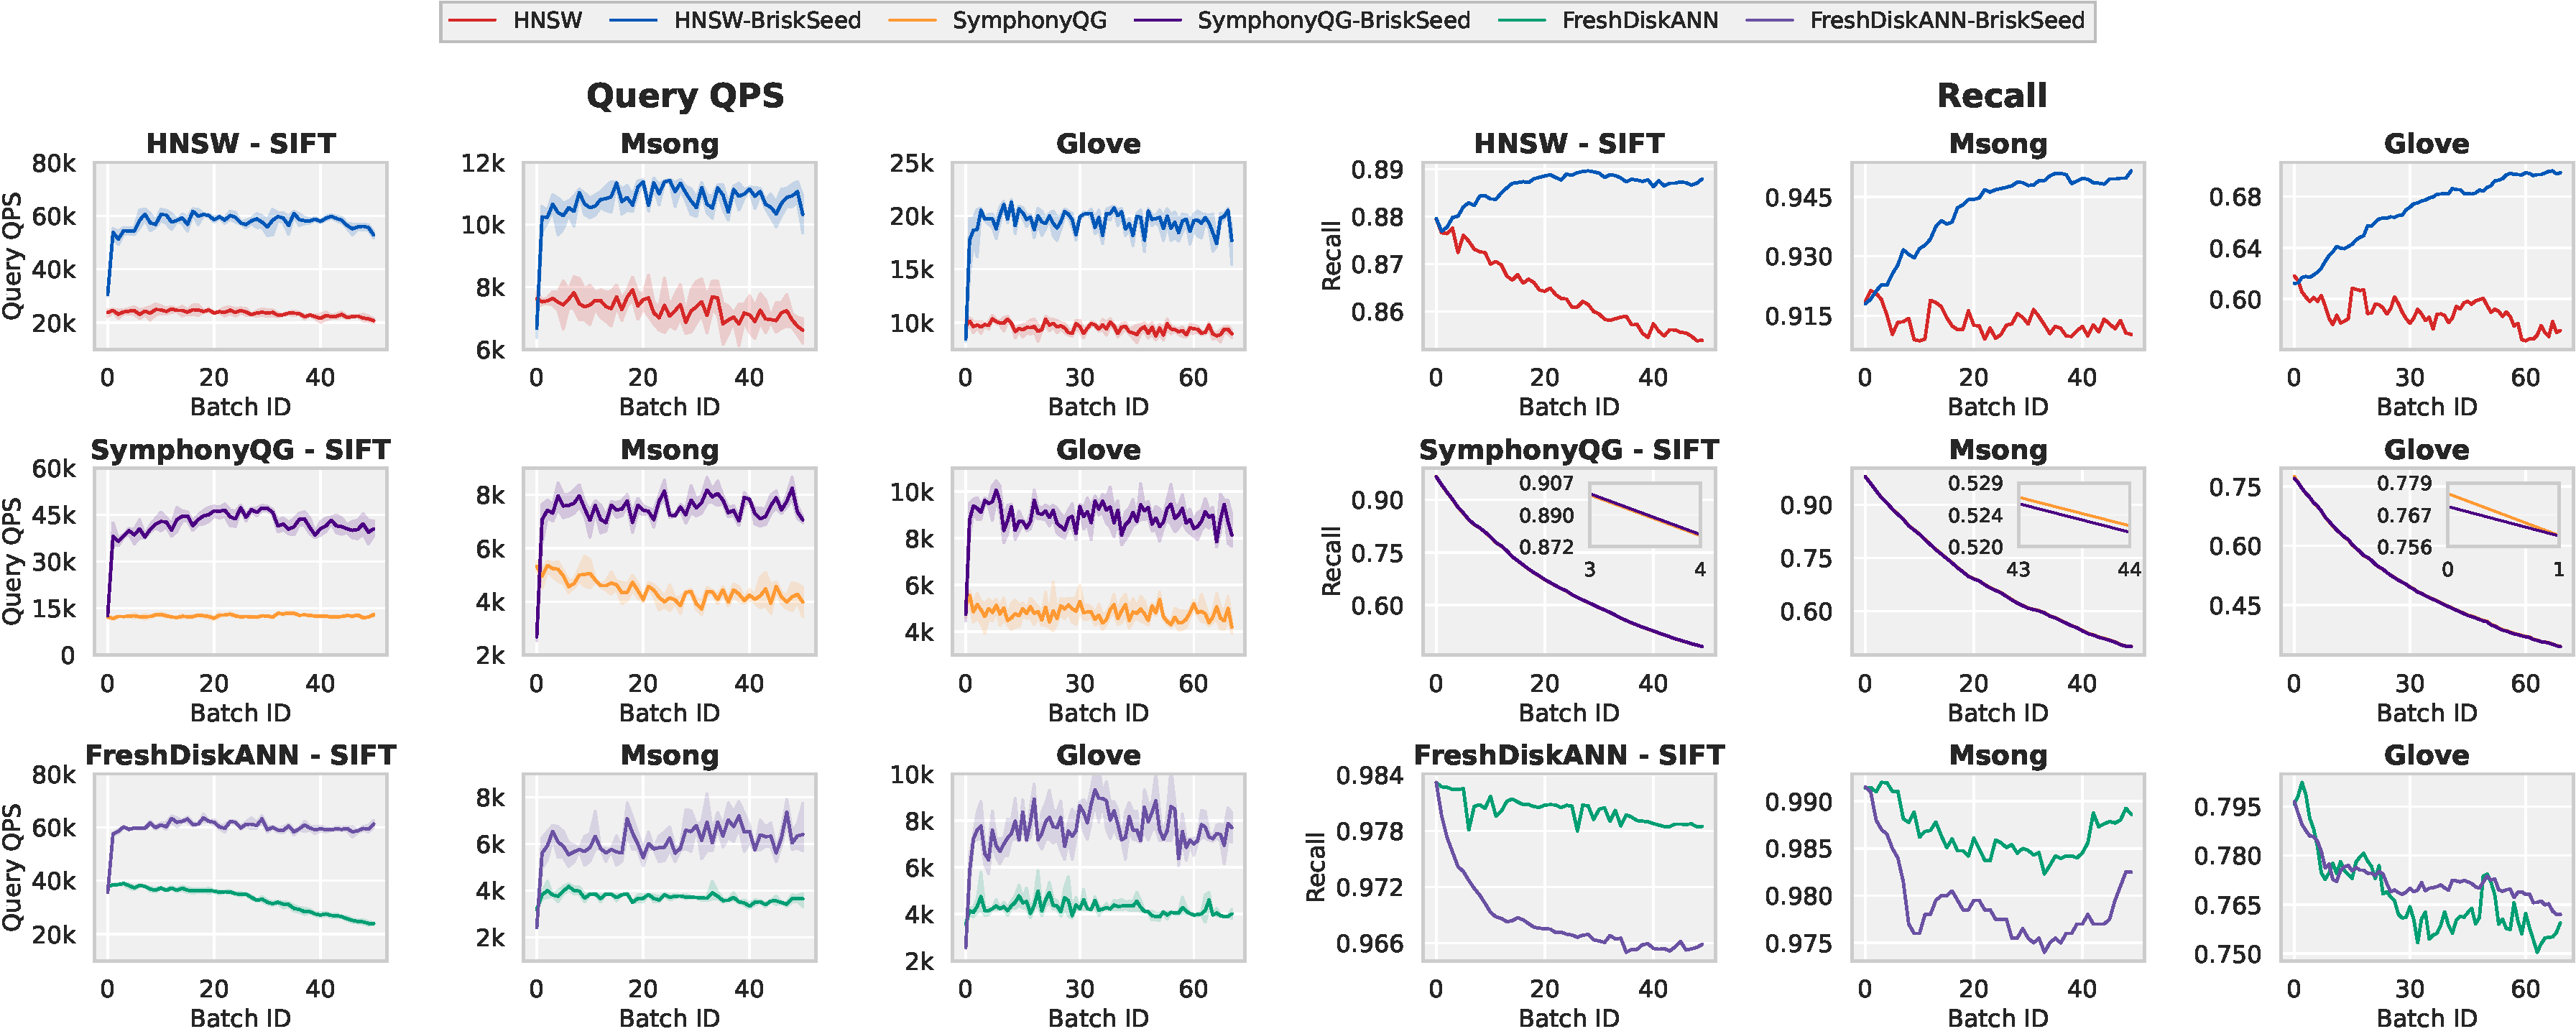
\includegraphics[width=\textwidth]{figures/qps_recall_all1.pdf}
\caption{QPS and Recall comparisons between baseline and baseline-\system on three datasets.}
\label{fig:qps-recall-three-datasets}
\end{figure*}


\subsection{Limitations}
The current implementation still leaves some limitations.
First, \system works best in common dynamic ANNS scenarios where the indexed database is large, and each update batch modifies only a small fraction of it, such as online recommendation.
When updates are large relative to the existing data, seed effectiveness may be significantly weakened, causing more fallbacks and limited speedups.
Second, the current prototype maintains seeds in memory and updates them online, but does not persist seed states on disks.
After a process restart, previously accumulated seed statistics are not retained.
Finally, \system currently targets single-node deployments; distributed seed placement and consistency across index partitions are left for future work.